% tikzpic.tex
\documentclass[crop,tikz]{standalone}% 'crop' is the default for v1.0, before it was 'preview'
%\usetikzlibrary{...}% tikz package already loaded by 'tikz' option
\usepackage{amsmath,amsthm,amssymb,mathrsfs,amsfonts,dsfont}

\begin{document}
    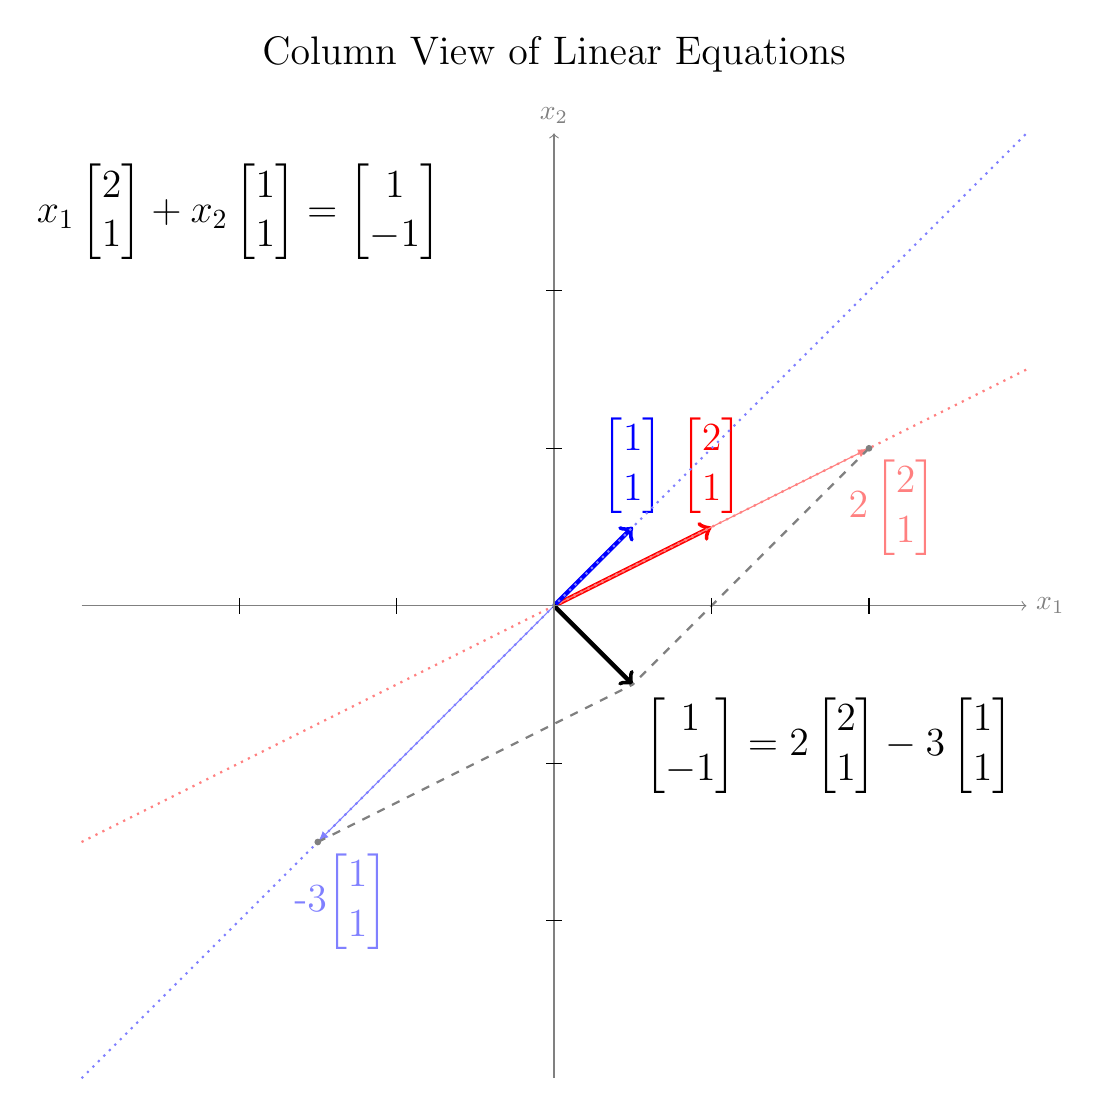
\begin{tikzpicture}[scale=1.0]
        % Text title saying "Column View"
        \node[font=\Large] at (0, 7) {Column View of Linear Equations};

        % Write down equation1.
        \node[font=\Large] at (-4, 5) {$x_1 \begin{bmatrix} 2 \\ 1\end{bmatrix} + x_2 \begin{bmatrix} 1 \\ 1\end{bmatrix} = \begin{bmatrix} 1 \\ -1\end{bmatrix}$};
        
        % Draw the column vector 1.
        \draw[red, ultra thick, ->] (0, 0) -- (2, 1) node[font=\Large, above] {$\begin{bmatrix} 2 \\ 1\end{bmatrix}$};
        \draw[red!50!, thin, -latex] (0, 0) -- (4, 2) node[font=\Large, below, xshift=0.3cm] {$2\begin{bmatrix} 2 \\ 1\end{bmatrix}$};
        \draw[red!50!, thick, dotted] (-6, -3) -- (6, 3);
        
        % Draw the column vector 2.
        \draw[blue, ultra thick, ->] (0, 0) -- (1, 1) node[font=\Large, above] {$\begin{bmatrix} 1 \\ 1\end{bmatrix}$};
        \draw[blue!50!, thin, -latex] (0, 0) -- (-3, -3) node[font=\Large, below, xshift=0.3cm] {-3$\begin{bmatrix} 1 \\ 1\end{bmatrix}$};
        \draw[blue!50!, thick, dotted] (-6, -6) -- (6, 6);
        
        % Draw the output vector.
        \draw[black, ultra thick, ->] (0, 0) -- (1, -1) node[font=\Large, below right] {$\begin{bmatrix} 1 \\ -1\end{bmatrix} = 2\begin{bmatrix} 2 \\ 1\end{bmatrix} - 3\begin{bmatrix} 1 \\ 1\end{bmatrix}$};
        
        % Plot the solution. 2 times column vector 1 minus 3 times column vector 2.
        \filldraw[gray] (4, 2) circle (1pt);
        \draw[gray, thick, dashed] (4, 2) -- (1, -1);
        \filldraw[gray] (-3, -3) circle (1pt);
        \draw[gray, thick, dashed] (-3, -3) -- (1, -1);
        
        
        \draw[->, gray] (-6,0) -- (6,0) node[right] {$x_1$};
        \draw[->, gray] (0,-6) -- (0,6) node[above] {$x_2$};
        \foreach \x in {-4,-2,2,4}
        \draw (\x,0.1) -- (\x,-0.1);
        \foreach \y in {-4,-2,2,4}
        \draw (0.1,\y) -- (-0.1,\y);
    \end{tikzpicture}
\end{document}